\documentclass[11pt,a4paper]{article}
\usepackage[margin=1in]{geometry}
\usepackage{booktabs}
\usepackage{listings}
\usepackage{xcolor}
\usepackage{hyperref}
\usepackage{amsmath}
\usepackage{amssymb}
\usepackage{tikz}
\usetikzlibrary{arrows.meta,positioning,shapes.geometric}

\lstset{
  basicstyle=\ttfamily\small,
  breaklines=true,
  frame=single,
  language=Python,
  keywordstyle=\color{blue},
  commentstyle=\color{gray}\itshape,
  showstringspaces=false
}

\title{DM--J4310--2EC V1.1 -- Cable-Drive Slack Removal\\
\large Low-Tension Winding: Theory and Implementation}
\author{}
\date{}

\begin{document}
\maketitle
\tableofcontents
\vspace{1em}

% =========================================================================
\section{Problem Statement}
\label{sec:problem}
% =========================================================================

Cable-driven robotic joints transmit force through tendons or Bowden cables.
Before a cable-drive robot can be operated, every cable must be pre-tensioned:
any slack must be wound out so that the cable lies straight and taut between
the drum and the distal attachment point.

This document describes the problem of \textbf{automatic slack removal} using
the DM-J4310-2EC motor as the cable drum actuator.  The goal is:

\begin{enumerate}
  \item Start with a wrapped but slack cable (the wrapping may be imprecise --
        the exact amount of slack is \emph{not known} in advance).
  \item Rotate the drum until the cable just becomes taut.
  \item Stop immediately -- do not overtension the cable or the distal joint.
\end{enumerate}

\noindent\textbf{Key constraints.}

\begin{itemize}
  \item The target shaft angle is \emph{unknown} -- position control requires
        a setpoint we do not have.
  \item Cable tension must not exceed the safe pre-tension limit (e.g.
        $\tau_\text{pre} \leq 0.5$\,N$\cdot$m at the drum) to avoid
        cable damage or joint overload.
  \item The algorithm must be self-terminating: it must stop even if the cable
        is already taut at startup (zero-slack case).
  \item A timeout must exist to prevent indefinite rotation if a cable is
        missing or disconnected.
\end{itemize}

% =========================================================================
\section{Control Mode Comparison}
\label{sec:modes}
% =========================================================================

The DM-J4310-2EC exposes three families of control modes over CAN.
Table~\ref{tab:modes} summarises their suitability for slack removal.

\begin{table}[ht]
\centering
\caption{CAN control modes vs.\ slack-removal suitability.}
\label{tab:modes}
\begin{tabular}{lllp{5cm}}
\toprule
Mode & CAN ID & Needs setpoint? & Suitability \\
\midrule
Position-Speed & $0\text{x}100 + \text{ID}$ & Yes ($p_\text{des}$ in rad)
  & \textbf{Poor.}  Target position unknown; overshooting overtensions cable. \\
Speed & $0\text{x}200 + \text{ID}$ & Yes ($v_\text{des}$ in rad/s)
  & \textbf{Moderate.}  Constant speed until stall; motor fights cable
    when taut; needs current monitoring to stop. \\
MIT Velocity & $\text{ID}$, $K_p=0$, $K_d>0$ & $\dot q_\text{des}$ (rad/s)
  & \textbf{Moderate.}  Similar to Speed mode; slightly easier to stop
    (velocity error grows at stall). \\
MIT Torque & $\text{ID}$, $K_p=0$, $K_d=0$ & $\tau_\text{ff}$ (N$\cdot$m)
  & \textbf{Best.}  Motor self-stalls when cable load equals $\tau_\text{ff}$;
    no overshoot; magnitude directly sets pre-tension. \\
\bottomrule
\end{tabular}
\end{table}

% =========================================================================
\section{Recommended Strategy: MIT Torque Mode with Stall Detection}
\label{sec:strategy}
% =========================================================================

\subsection{Physical intuition}

\begin{figure}[ht]
\centering
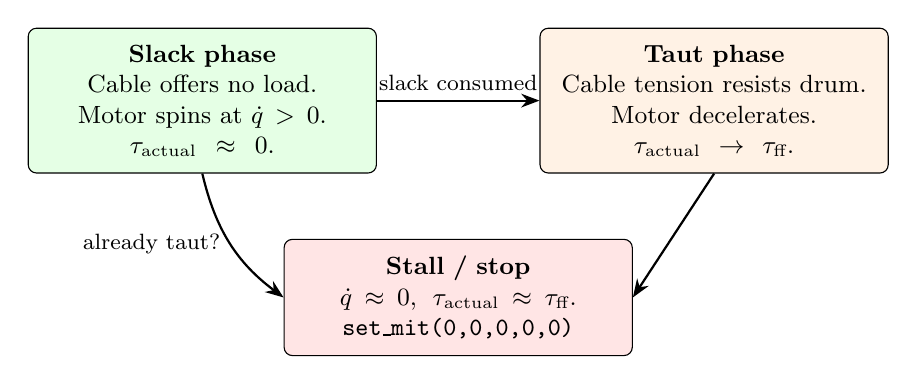
\begin{tikzpicture}[every node/.style={font=\small}, scale=1.0]
  % Slack phase
  \node[draw, rounded corners=3pt, fill=green!10, text width=4cm,
        align=center, minimum height=1.2cm, inner sep=6pt] (slack) at (0,0) {
    \textbf{Slack phase}\\
    Cable offers no load.\\
    Motor spins at $\dot q > 0$.\\
    $\tau_\text{actual} \approx 0$.
  };
  % Taut phase
  \node[draw, rounded corners=3pt, fill=orange!10, text width=4cm,
        align=center, minimum height=1.2cm, inner sep=6pt] (taut)
    at (6.5,0) {
    \textbf{Taut phase}\\
    Cable tension resists drum.\\
    Motor decelerates.\\
    $\tau_\text{actual} \to \tau_\text{ff}$.
  };
  % Stall
  \node[draw, rounded corners=3pt, fill=red!10, text width=4cm,
        align=center, minimum height=1.2cm, inner sep=6pt] (stall)
    at (3.25,-2.5) {
    \textbf{Stall / stop}\\
    $\dot q \approx 0$,\;
    $\tau_\text{actual} \approx \tau_\text{ff}$.\\
    \texttt{set\_mit(0,0,0,0,0)}
  };
  \draw[-Stealth, thick] (slack.east) -- node[above, font=\footnotesize]
    {slack consumed} (taut.west);
  \draw[-Stealth, thick] (taut.south) -- (stall.east);
  \draw[-Stealth, thick] (slack.south) to[bend right=20]
    node[left, font=\footnotesize] {already taut?} (stall.west);
\end{tikzpicture}
\caption{Phase diagram of the slack-removal procedure.  MIT torque mode
naturally transitions from the slack phase to a stall when cable tension
equals $\tau_\text{ff}$.}
\label{fig:phases}
\end{figure}

In MIT torque mode ($K_p = K_d = 0$,\; $\tau_\text{ff} > 0$) the motor
applies a constant torque to the drum.  The torque balance on the drum shaft
is:

\[
  J\,\ddot{q} = \tau_\text{ff} - \tau_\text{friction} - \tau_\text{cable}
\]

where $\tau_\text{cable} = r \cdot T$ is the moment of cable tension $T$ on
a drum of effective radius $r$.

\begin{itemize}
  \item \textbf{Slack}: $\tau_\text{cable} \approx 0$, so $\ddot q > 0$ and
        the motor accelerates until $\tau_\text{friction}$ limits it.
  \item \textbf{Transition}: as the last slack is wound onto the drum, $T$
        rises rapidly.
  \item \textbf{Taut}: $\tau_\text{cable}$ rises until
        $\tau_\text{cable} \geq \tau_\text{ff} - \tau_\text{friction}$,
        at which point $\ddot q \leq 0$ and the motor decelerates.
  \item \textbf{Stall}: $\dot q = 0$.  The motor holds the cable at tension
        $T = \tau_\text{ff}/r$ and draws no further current (static stall).
\end{itemize}

This means $\tau_\text{ff}$ \emph{directly controls the pre-tension}
applied to the cable at the moment of stopping -- which is the most important
design parameter for cable-driven robots.

\subsection{Stall detection criteria}

Two independent signals are available from the DM-J4310-2EC CAN feedback:
$\dot q$ (velocity, rad/s) and $\tau_\text{est}$ (estimated torque, N$\cdot$m).
Using both together avoids false triggers:

\begin{enumerate}
  \item \textbf{Velocity criterion}: $|\dot q| < \varepsilon_v$ for a sustained
        duration $\Delta t_\text{stall}$.  A single momentary slowdown (slack
        loop, knot passing) does not trigger a stop; the motor must be
        continuously stalled for $\Delta t_\text{stall}$.
  \item \textbf{Torque criterion} (optional cross-check):
        $\tau_\text{est} > \tau_\text{taut}$, confirming actual load on the cable
        rather than a loose mechanical jam that stalls without tensioning.
\end{enumerate}

The algorithm uses criterion~1 as the primary stop condition and
criterion~2 as a guard to reject false stalls at startup (friction stall
before cable is wound).

\subsection{State machine}
\label{sec:statemachine}

\begin{figure}[ht]
\centering
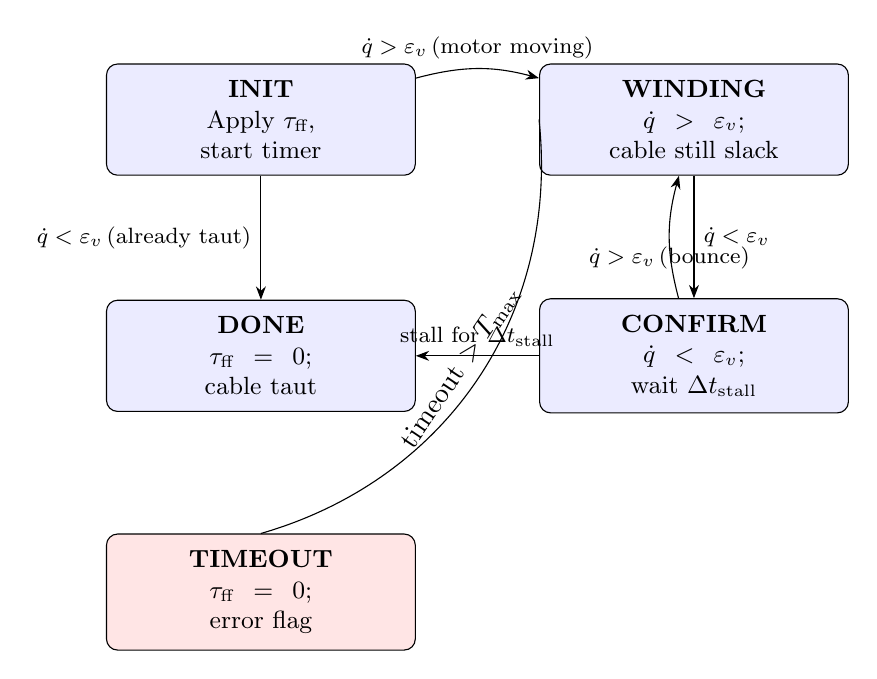
\begin{tikzpicture}[
    state/.style={draw, rounded corners=4pt, fill=blue!8,
                  text width=3.5cm, align=center, minimum height=1.2cm,
                  inner sep=6pt, font=\small},
    every edge/.style={draw, -Stealth, font=\footnotesize}
  ]
  \node[state] (INIT)    at (0,   0) {\textbf{INIT}\\Apply $\tau_\text{ff}$,\\start timer};
  \node[state] (WINDING) at (5.5, 0) {\textbf{WINDING}\\$\dot q > \varepsilon_v$;\\cable still slack};
  \node[state] (CONFIRM) at (5.5,-3) {\textbf{CONFIRM}\\$\dot q < \varepsilon_v$;\\wait $\Delta t_\text{stall}$};
  \node[state] (DONE)    at (0,  -3) {\textbf{DONE}\\$\tau_\text{ff} = 0$;\\cable taut};
  \node[state, fill=red!10] (TIMEOUT) at (0,-6) {\textbf{TIMEOUT}\\$\tau_\text{ff} = 0$;\\error flag};

  \draw (INIT) edge[bend left=15] node[above] {$\dot q > \varepsilon_v$\,(motor moving)} (WINDING);
  \draw (INIT) edge node[left] {$\dot q < \varepsilon_v$\,(already taut)} (DONE);
  \draw (WINDING) edge node[right] {$\dot q < \varepsilon_v$} (CONFIRM);
  \draw (CONFIRM) edge[bend left=15] node[below] {$\dot q > \varepsilon_v$\,(bounce)} (WINDING);
  \draw (CONFIRM) edge node[above] {stall for $\Delta t_\text{stall}$} (DONE);
  \draw (WINDING.west) to[bend left=40] node[above, sloped]
    {timeout $>T_\text{max}$} (TIMEOUT.north);
\end{tikzpicture}
\caption{State machine for the slack-removal algorithm.}
\label{fig:fsm}
\end{figure}

% =========================================================================
\section{Parameter Selection}
\label{sec:params}
% =========================================================================

\subsection{Winding torque $\tau_\text{ff}$}

The winding torque serves two simultaneous roles: it must be large enough to
overcome bearing friction and cable bending stiffness, but small enough to
set a safe cable pre-tension.

\[
  \tau_\text{ff} \;=\; r \cdot T_\text{pre} + \tau_\text{friction}
\]

For the DM-J4310-2EC ($\text{TMAX} = 10$\,N$\cdot$m at output shaft):

\begin{table}[ht]
\centering
\caption{Recommended $\tau_\text{ff}$ ranges.}
\label{tab:tau}
\begin{tabular}{lll}
\toprule
Application & $\tau_\text{ff}$ (N$\cdot$m) & Notes \\
\midrule
Lightweight finger tendon ($r \approx 5$\,mm, $T < 10$\,N)
  & 0.05\,--\,0.15 & Very gentle; friction may dominate \\
Forearm/wrist cable ($r \approx 10$\,mm, $T < 30$\,N)
  & 0.15\,--\,0.40 & Typical cable-drive pre-tension \\
Upper-arm / large joint ($r \approx 20$\,mm, $T < 50$\,N)
  & 0.40\,--\,1.00 & Verify cable safe working load \\
\bottomrule
\end{tabular}
\end{table}

\noindent\textbf{Rule of thumb}: start at $\tau_\text{ff} = 0.2$\,N$\cdot$m and
increase until the motor reliably moves against the cable bending stiffness.
Never exceed the cable's rated safe working load.

\subsection{Stall velocity threshold $\varepsilon_v$}

Choose $\varepsilon_v$ such that it is above measurement noise but well below
any meaningful winding speed.  For the J4310-2EC's 14-bit encoder,
the velocity resolution at 1\,kHz is about $0.01$\,rad/s.

\[
  \varepsilon_v \approx 0.05\text{--}0.15\;\mathrm{rad/s}
\]

\subsection{Stall confirmation time $\Delta t_\text{stall}$}

A short burst of reduced velocity (e.g.\ a cable knot passing the drum)
should not trigger a stop.  Set:
\[
  \Delta t_\text{stall} \approx 0.25\text{--}0.5\;\mathrm{s}
\]

\subsection{Safety timeout $T_\text{max}$}

Protects against a disconnected or missing cable.  Set to the maximum
expected winding time:
\[
  T_\text{max} = \frac{L_\text{slack,max}}{r \cdot \bar{\dot{q}}}
\]

For example: 0.3\,m slack, 10\,mm drum radius, 1\,rad/s winding speed
$\Rightarrow T_\text{max} \approx 30$\,s.  The default in the test script
is \texttt{TIMEOUT\_S = 20.0}.

% =========================================================================
\section{Implementation Notes for DM-J4310-2EC}
\label{sec:impl}
% =========================================================================

\subsection{Torque feedback caveat}

The firmware's torque estimate ($\tau_\text{est}$) is derived from
phase current and is noisy at low loads.  Below $\approx 0.1$\,N$\cdot$m
the signal is not reliable for thresholding.  Therefore the primary stop
criterion uses \emph{velocity} (reliable), and torque is used only as an
optional cross-check when $\tau_\text{ff} \geq 0.3$\,N$\cdot$m.

\subsection{Winding direction}

The sign of $\tau_\text{ff}$ must match the cable-winding direction.
Use a positive value if the cable winds when the output shaft rotates
counter-clockwise when viewed from the encoder end (the default J4310
convention).  Verify by commanding a tiny torque and observing which
direction the motor moves.

\subsection{Post-stall hold}

After stall detection, the script has two options:

\begin{enumerate}
  \item \textbf{Release} (\texttt{TAU\_FF = 0}): motor becomes free.
        The cable may relax slightly due to elasticity.  Use when the
        distal attachment is passive (spring-tensioned).
  \item \textbf{Hold with low-stiffness position control}
        ($K_p \approx 5$, $K_d \approx 0.5$, $q_\text{des} = q_\text{stall}$):
        maintains the drum angle to preserve cable tension.
        Use when the cable must stay taut for subsequent operation.
\end{enumerate}

The test script (Section~\ref{sec:testscript}) supports both via the
\texttt{POST\_STALL\_HOLD} flag.

\subsection{Output-shaft units}

All CAN values are in \textbf{output-shaft units}: radians, rad/s, N$\cdot$m.
The 10:1 gearbox is transparent -- the firmware uses the output-shaft encoder
directly.  Do \emph{not} multiply torques or velocities by the gear ratio.

\subsection{Winding speed (free-spin)}

In MIT torque mode the winding speed is not commanded directly -- it is
determined by the balance of $\tau_\text{ff}$ minus friction.  Typical
free-spinning velocity for $\tau_\text{ff} = 0.3$\,N$\cdot$m is
3\,--\,8\,rad/s at the output shaft.  If this is too fast for the cable
mechanism, use MIT velocity mode instead (Section~\ref{sec:velmode}).

% =========================================================================
\section{Alternative: MIT Velocity Mode with Torque Monitoring}
\label{sec:velmode}
% =========================================================================

If a controlled winding speed is required (e.g.\ a Bowden sheath that could
kink), use MIT velocity mode ($K_p = 0$, $K_d > 0$, $\dot q_\text{des}$
small) and monitor the torque estimate:

\begin{itemize}
  \item Set $\dot q_\text{des} = 0.5$\,--\,2.0\,rad/s (slow, controlled).
  \item Monitor $\tau_\text{est}$: when $\tau_\text{est} > \tau_\text{taut}$
        for $\Delta t_\text{stall}$, cable is taut.
  \item Stop and optionally switch to position hold.
\end{itemize}

Limitation: the velocity loop fights the cable when taut, potentially
applying larger forces than needed.  A low $K_d$ (0.3\,--\,0.8) reduces this.

% =========================================================================
\section{Test Script: \texttt{11\_cable\_wind\_to\_tension.py}}
\label{sec:testscript}
% =========================================================================

The script \texttt{tests/damiao/11\_cable\_wind\_to\_tension.py} implements
the state machine of Section~\ref{sec:statemachine} using the
\texttt{DamiaoBus} context manager.

\subsection{Configurable parameters (top of script)}

\begin{lstlisting}
# ---- tuning --------------------------------------------------------
TAU_FF         = 0.3    # N.m  winding torque (positive = CCW drum)
V_STALL_EPS    = 0.10   # rad/s  below this -> treat as stalled
T_STALL_CONFIRM= 0.35   # s  must be stalled this long to confirm
TAU_TAUT_MIN   = 0.15   # N.m  torque must exceed this during stall
TIMEOUT_S      = 20.0   # s  abort if not taut within this time
WINDING_HZ     = 100    # Hz control loop rate
POST_STALL_HOLD= True   # True -> hold drum angle after taut
KP_HOLD        = 5.0    # spring for post-stall hold (if enabled)
KD_HOLD        = 0.5    # damping for post-stall hold
\end{lstlisting}

\subsection{State machine output}

\begin{lstlisting}[language={}]
[cable_wind] State: INIT  | q=+0.00 rad  dq=+0.00 rad/s  tau=+0.00 Nm
[cable_wind] State: WINDING| q=+0.12 rad  dq=+3.42 rad/s  tau=+0.04 Nm
...
[cable_wind] State: CONFIRM| q=+2.18 rad  dq=+0.02 rad/s  tau=+0.28 Nm
[cable_wind] DONE: cable taut at q=+2.18 rad after 0.72 s.
[cable_wind] Holding drum angle q=+2.18 rad with Kp=5.0, Kd=0.5
\end{lstlisting}

\subsection{Safety notes}

\begin{itemize}
  \item \textbf{Power on the motor before running the script.}
        The script enables the motor on entry.
  \item \textbf{Keep the cable force path clear.}  Ensure the distal
        attachment is secure before running.
  \item \textbf{Ctrl+C} will stop the motor immediately (zero torque sent
        in the \texttt{finally} block).
  \item \textbf{Do not set} \texttt{TAU\_FF} \textbf{above the cable's safe
        working load divided by the drum radius.}
\end{itemize}

% =========================================================================
\section{Quick Reference}
\label{sec:quickref}
% =========================================================================

\begin{table}[ht]
\centering
\caption{Parameter quick reference for \texttt{11\_cable\_wind\_to\_tension.py}.}
\begin{tabular}{llll}
\toprule
Parameter & Default & Unit & When to change \\
\midrule
\texttt{TAU\_FF} & 0.3 & N$\cdot$m & Adjust for cable pre-tension target \\
\texttt{V\_STALL\_EPS} & 0.10 & rad/s & Increase in noisy environments \\
\texttt{T\_STALL\_CONFIRM} & 0.35 & s & Increase if false triggers occur \\
\texttt{TAU\_TAUT\_MIN} & 0.15 & N$\cdot$m & Raise if $\tau_\text{ff}$ is large \\
\texttt{TIMEOUT\_S} & 20.0 & s & Set to max expected winding time \\
\texttt{POST\_STALL\_HOLD} & True & bool & False = release after taut \\
\texttt{KP\_HOLD} & 5.0 & -- & Stiffen to resist distal forces \\
\texttt{KD\_HOLD} & 0.5 & -- & Increase to damp hold oscillations \\
\bottomrule
\end{tabular}
\end{table}

\end{document}
